\newcommand{\baselineEvalFigure}{
\begin{figure}[t]
    \centering
    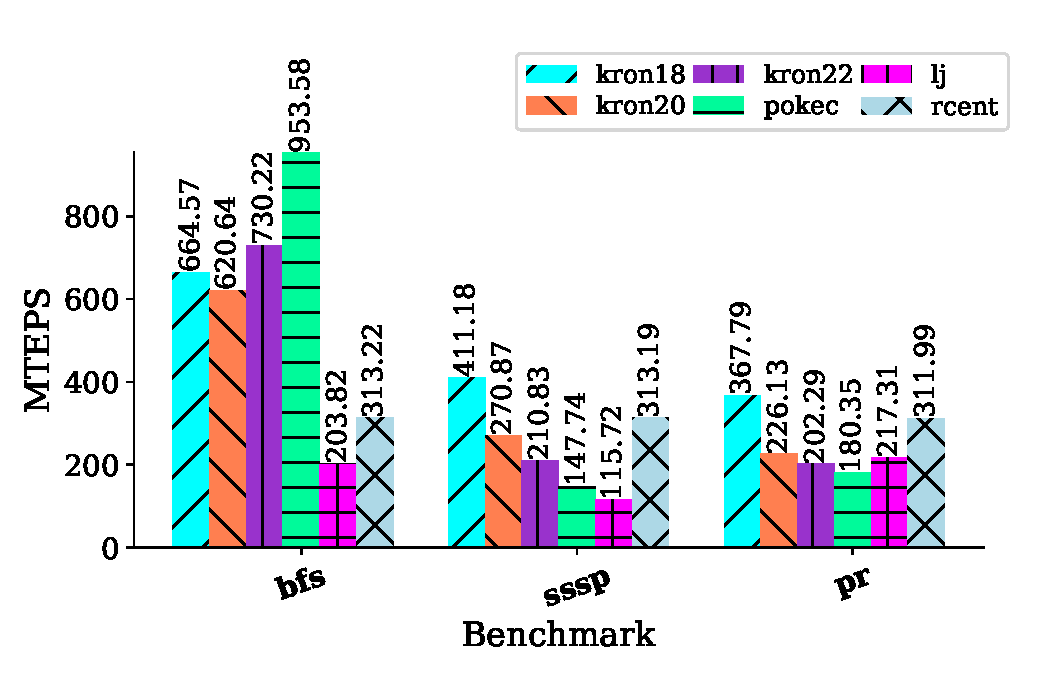
\includegraphics[scale = 0.5]{graphit-figures/baseline.pdf}
    \caption{Baseline code generation results for each benchmark in the dense pull direction with no manycore specific optimizations.}
    \label{pap:generals:sec:eval:fig:baseline}
\end{figure}
}

\newcommand{\pushEvalFigure}{
\begin{figure}[t]
    \centering
    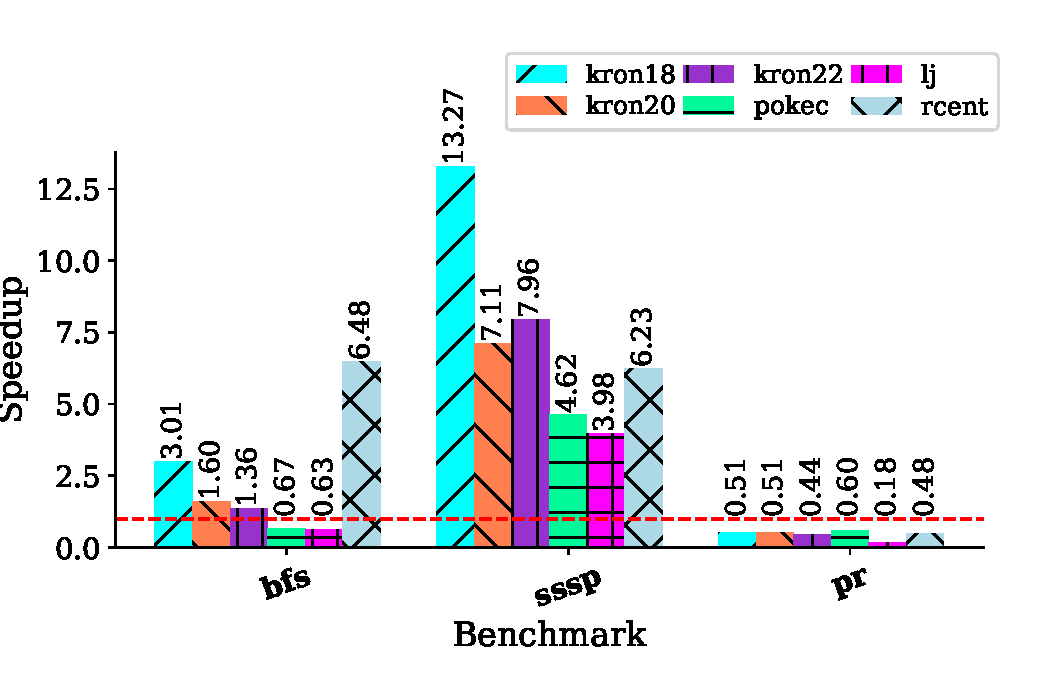
\includegraphics[scale = 0.5]{graphit-figures/push.pdf}
    \caption{Baseline code generation results for each benchmark in the push direction with no manycore specific optimizations.}
    \label{pap:generals:sec:eval:fig:push}
\end{figure}
}

\newcommand{\edgeSpeedupFigure}{
\begin{figure}[t]
    \centering
    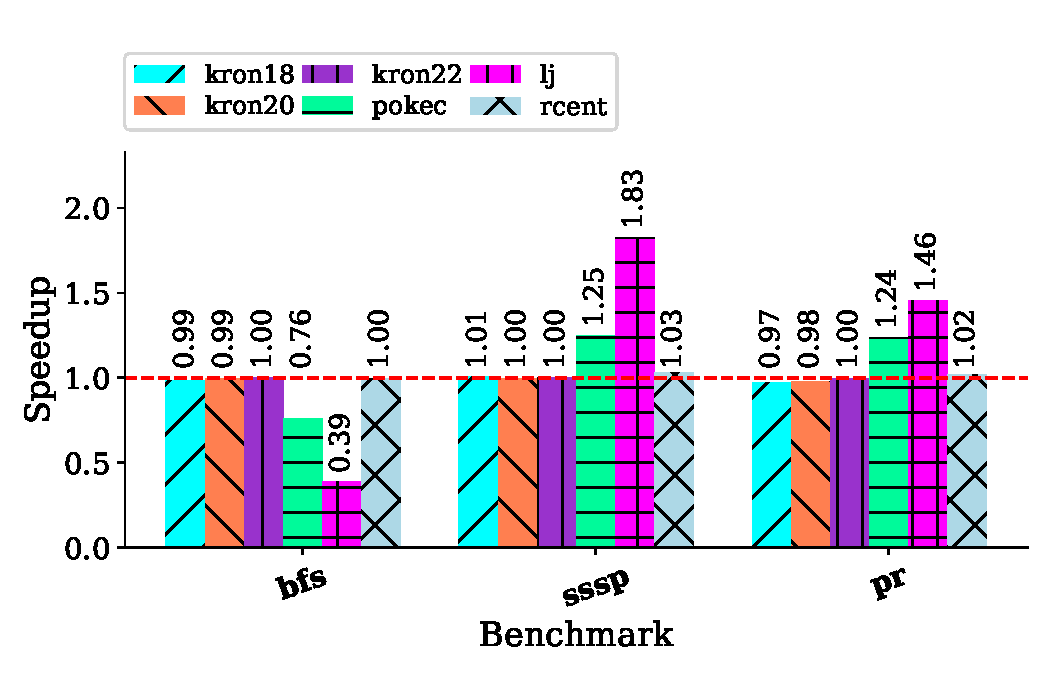
\includegraphics[scale = 0.5]{graphit-figures/edge.pdf}
    \caption{Speedup results for edge based optimization over the baseline dense pull implementation for each benchmark.}
    \label{pap:generals:sec:eval:fig:edge}
    \vspace{-2mm} 
\end{figure}
}

\newcommand{\blockBFSFigure}{
\begin{figure}[t]
    \centering
    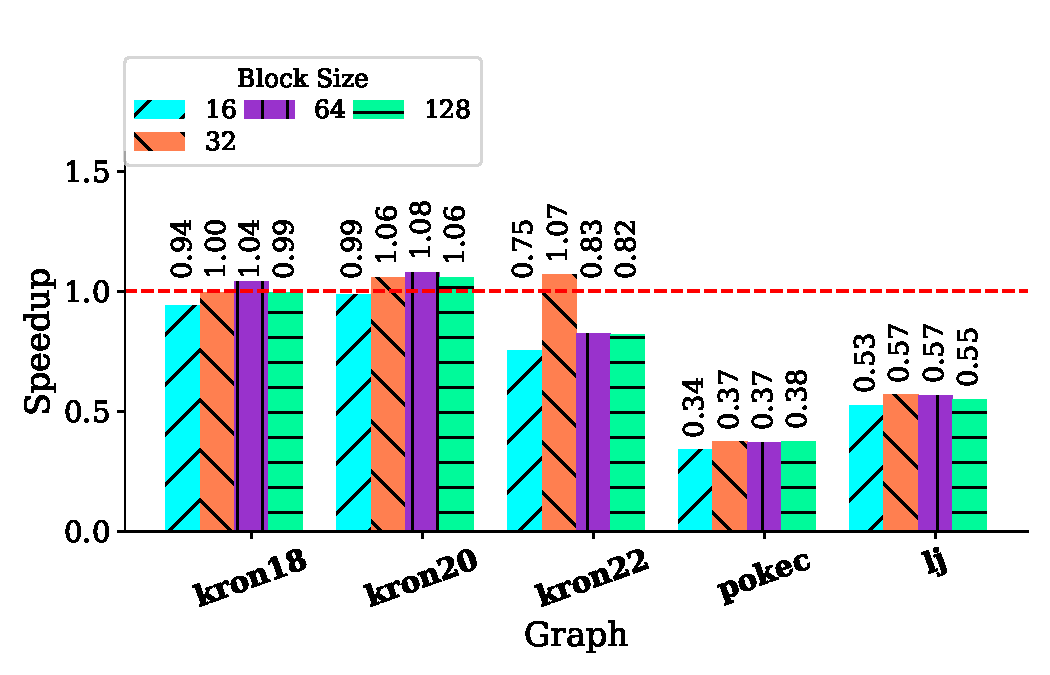
\includegraphics[scale = 0.5]{graphit-figures/bfs-block.pdf}
    \caption{MTEPS results for varying block sizes using the blocked access method on BFS.}
    \label{pap:generals:sec:eval:fig:bfsblock}
\end{figure}
}

\newcommand{\blockSSSPFigure}{
\begin{figure}[t]
    \centering
    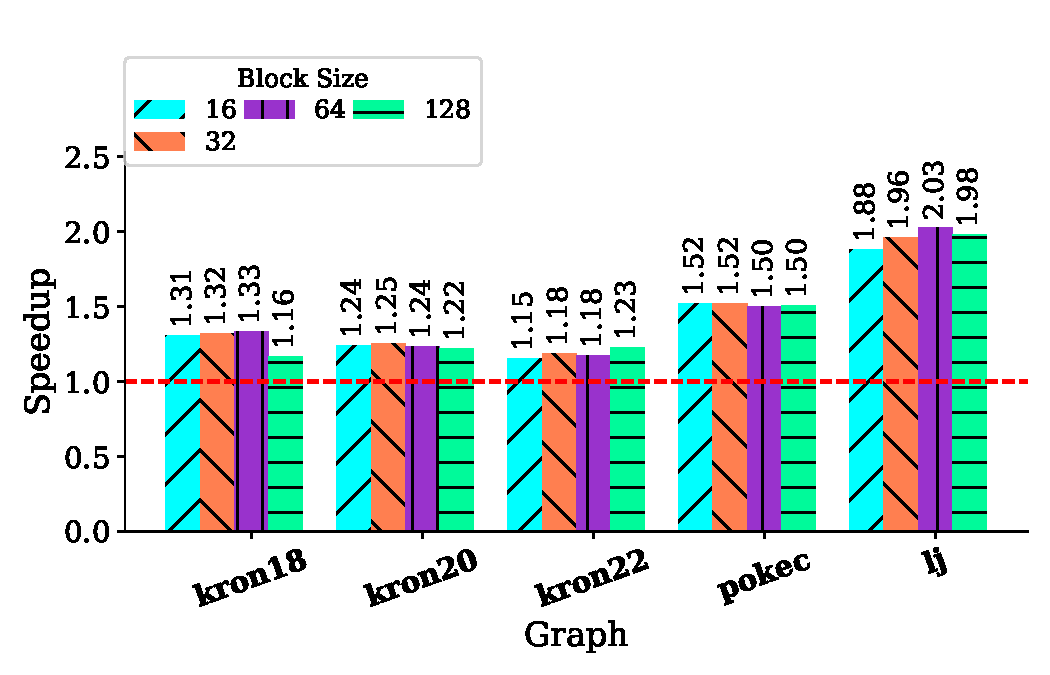
\includegraphics[scale=0.5]{graphit-figures/sssp-block.pdf}
    \caption{Speedup results for varying block sizes using the blocked access method on SSSP. Speedup is calculated over the baseline pull direction implementation.}
    \label{pap:generals:sec:eval:fig:ssspblock}
\end{figure}
}

\newcommand{\cacheBFSFigure}{
\begin{figure}[t]
    \centering
    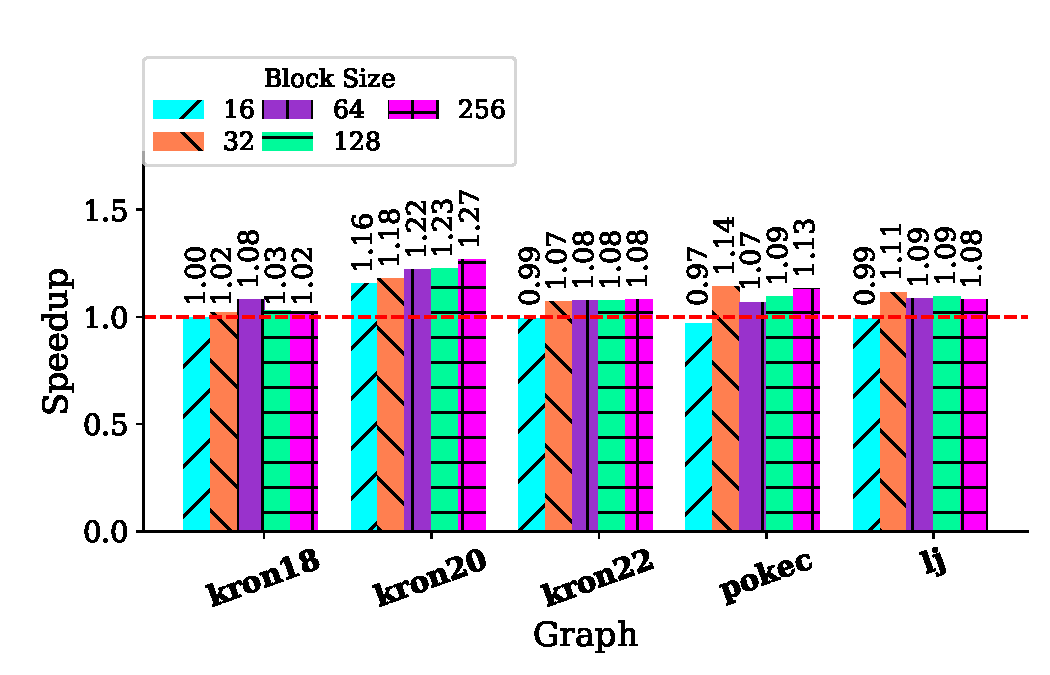
\includegraphics[scale = 0.5]{graphit-figures/bfs-cache.pdf}
    \caption{MTEPS results for varying work block sizes using the manycore aware vertex partitioning scheme on BFS.}
    \label{pap:generals:sec:eval:fig:bfscache}
\end{figure}
}

\newcommand{\cacheSSSPFigure}{
\begin{figure}[t]
    \centering
    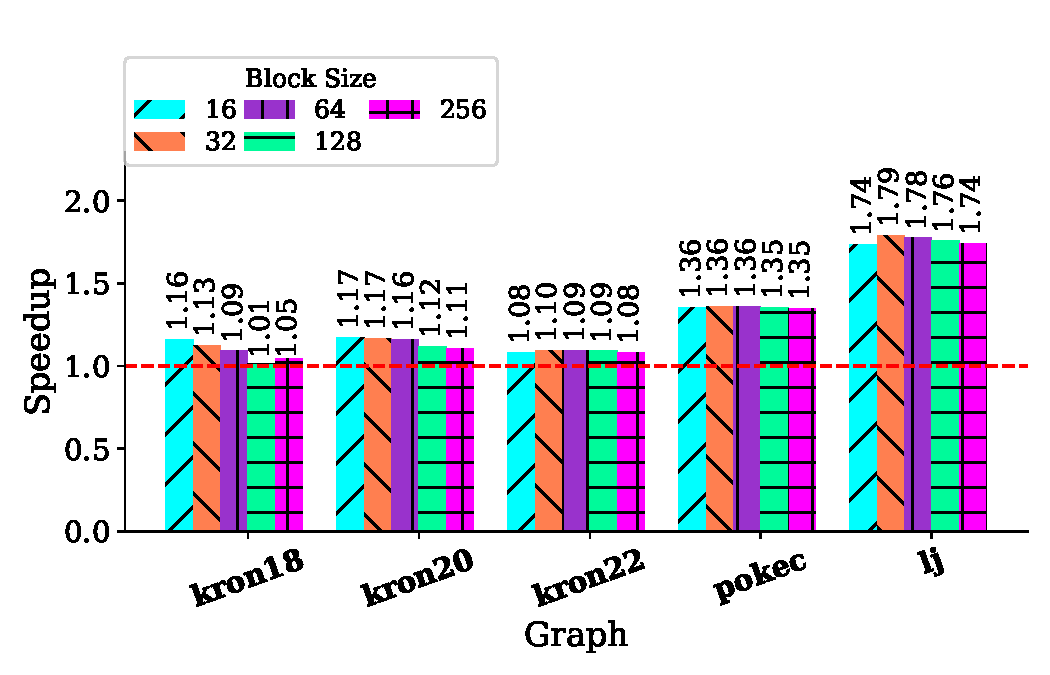
\includegraphics[scale=0.5]{graphit-figures/sssp-cache.pdf}
    \caption{Speedup results for varying work block sizes using the manycore aware vertex partitioning scheme on SSSP. Speedup is calculated over the baseline pull direction implementation.}
    \label{pap:generals:sec:eval:fig:ssspcache}
\end{figure}
}

\newcommand{\allBlockedFigure}{
\begin{figure}[t]
    \centering
    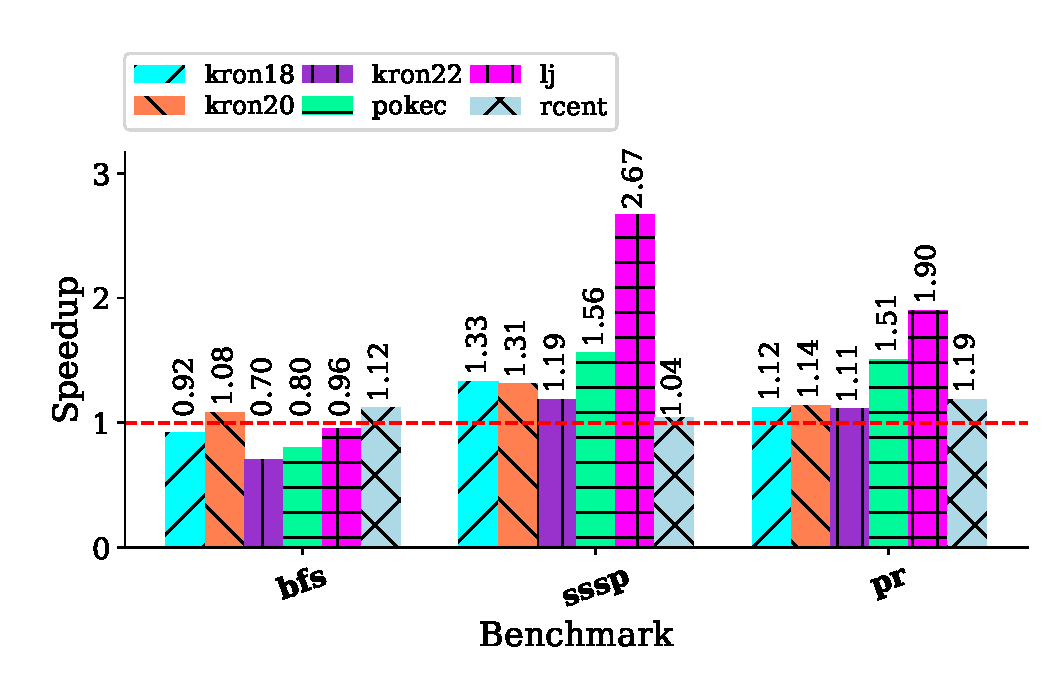
\includegraphics[scale = 0.5]{graphit-figures/all-blocked.pdf}
    \caption{Blocked access method speedup results for each benchmark. Speedup is calculated over the baseline pull direction implementation.} %For each graph and benchmark, block sizes of 16, 32, 64, and 128 elements were tested and the best performing block size is reported here.
    \label{pap:generals:sec:eval:fig:blocked}
\end{figure}
}

\newcommand{\allAlignedFigure}{
\begin{figure}[t]
    \centering
    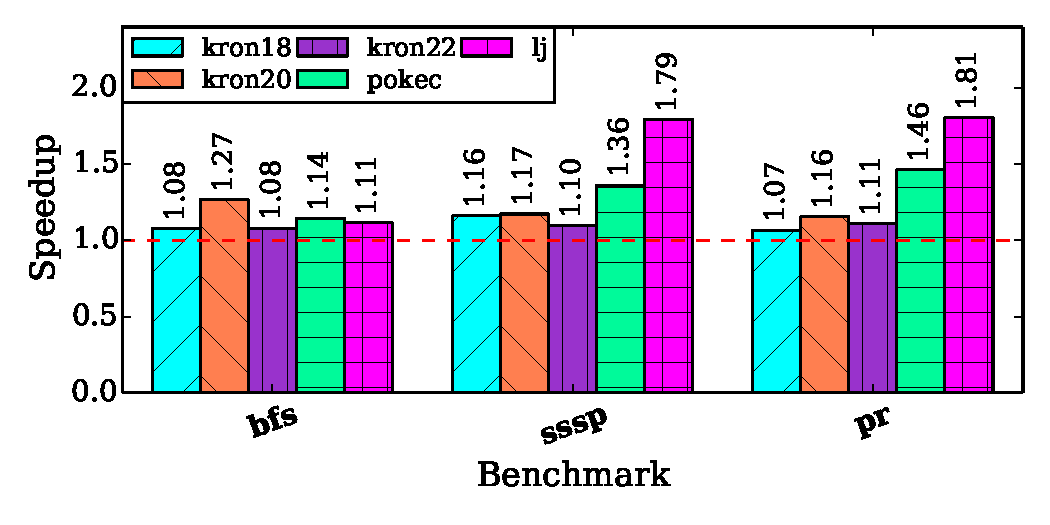
\includegraphics[scale = 0.5]{graphit-figures/align.pdf}
    \caption{Alignment-based partitioning speedup results for each benchmark. Speedup is calculated over the baseline pull direction implementation.} %For each graph and benchmark, work group sizes of 16, 32, 64, 128, and 256 vertices were tested and the best performing work group size is reported here.
    \label{pap:generals:sec:eval:fig:aligned}
    \vspace{-2mm} 
\end{figure}
}

%I am not sure if this is the best way to present an overview of results or if we need it. 
\newcommand{\overviewResultsTable}{
\begin{table}[]
\centering
\begin{tabular}{lrcl}
%\hline
\toprule
\textbf{Benchmark} & \textbf{Graph} & \textbf{MTEPS} & \textbf{Optimization} \\ \midrule
 \multirow{5}{*}{BFS}& kron18 & 457.09 & Cache-Aligned \pull \\ %\cline{2-4}
 & kron20 & 296.32 & Cache-Aligned \pull \\ %cline{2-4}
 & kron22 & 241.95 & Cache-Aligned \pull \\ %\cline{2-4}
 & pokec & 148.02 &  Cache-Aligned \pull\\ %\cline{2-4}
 & lj & 304.36 & Cache-Aligned \pull \\ \hline
 \multirow{5}{*}{PR}& kron18 & 412.34 & Blocked \pull \\ %\cline{2-4}
 & kron20 & 261.35 & Cache-Aligned \pull \\ %\cline{2-4}
 & kron22 & 224.88 & Blocked \pull \\ %\cline{2-4}
 & pokec & 272.57 & Blocked \pull \\ %\cline{2-4}
 & lj & 413.06 & Blocked \pull \\ \hline
 \multirow{5}{*}{SSSP}& kron18 & 467.08 & Cache-Aligned \pull \\ %\cline{2-4}
 & kron20 & 364.36& Baseline \push \\ %\cline{2-4}
 & kron22 & 404.27 & Baseline \push \\ %\cline{2-4}
 & pokec & 149.17 & Cache-Aligned \pull \\ %\cline{2-4}
 & lj & 268.87 & Cache-Aligned \pull \\ %\hline
 \bottomrule
\end{tabular}
\caption{Table containing best MTEPS results across all benchmarks and input graphs. The optimizations used to achieve these results are also listed above.}
\label{pap:generals:sec:eval:tab:overview}
\end{table}
}

\newcommand{\relatedMTEPSTable}{
\begin{table}[]
\centering
\begin{tabular}{cllll}
%\hline
\toprule
 \textbf{Source} & \textbf{Platform} & \textbf{Benchmark} & \textbf{Graph}  & \textbf{MTEPS} \\ \midrule
 \cite{slota2015high}& Xeon Phi MIC & CC & LJ (22) & 240 \\ %\hline
 \cite{slota2015high}& Xeon Phi MIC & CC & Flickr (19) & 140\\ %\hline
 %Galois \cite{aasawat2018well}& Ivy Bridge & PR & LJ (22) & 207.67 \\ \hline
 \cite{khorasani2014cusha} & GTX780 & BFS & LJ (22) & 272.4 \\ %\hline
 \cite{zhong2013medusa}& C2050 & BFS & KKT (21) & 351.5 \\ %\hline
 \cite{yang2019graphblast}& k40c & SSSP & LJ (22) & 334.2 \\ %\hline
 \cite{wang2016gunrock} & k40c & SSSP & LJ (22) & 217.9 \\
 \bottomrule

\end{tabular}
\caption{Performance results in MTEPS from other graph processing frameworks. The benchmark CC is strongly connected components.}
\label{sec:related:tab:mteps}
\vspace{-1mm} 
\end{table}
}
\newcommand{\graphInfoTable}{
\begin{table}[]
\centering
\begin{tabular}{c|c|c|c}
%\hline
 \textbf{Name} & \textbf{Scale} & \textbf{\# Vertices} & \textbf{\# Edges} \\ \hline %\hline
 kron18 & 18 & 262,144 & 4,194,304 \\ \hline
 kron20 & 20 & 1,048,576 & 16,777,216 \\ \hline
 kron22 & 22 & 4,194,304 & 67,108,864 \\ \hline
 pokec & 20.5 & 1,632,803 & 30,622,564 \\ \hline
 livejournal (lj) & 22 & 3,997,962 & 34,681,189 \\ %\hline
\end{tabular}

\caption{The vertex and edge information for each of the graphs used in our evaluation. We use synthetic \kron graphs used in the Graph500 benchmark and two real world graphs.}
\label{sec:eval:tab:graphs}
\end{table}
}